\documentclass[12pt]{article}
\usepackage[utf8]{inputenc}
\usepackage{amsmath}
\usepackage{systeme}
\usepackage{amsfonts}
\usepackage{graphicx}
\usepackage{enumitem}
\usepackage{hyperref}
\usepackage{xcolor}
\usepackage{kbordermatrix}
\usepackage{centernot}
\usepackage{xcolor}
\usepackage{amsmath,amssymb,amsthm}

\title{%
	\textbf{Notițe Seminar 10, 11}}

\begin{document}
	
	\maketitle
	
	\textbf{{Intro:}} După cum știți, de săptămâna trecută am început capitolul de \textbf{Clusterizare}. Mai concret, am făcut clusterizare \textbf{ierarhică}. De acum începem clusterizarea \textbf{neierarhică}. Mai concret, în următoarele două seminarii vom face algoritmul \textbf{k-means}.
	
	\section{k-means - noțiuni de bază}
	
	$k$ va fi un număr natural nenul care va semnifica în câte grupuri/clustere vrem să împărțim instanțele.
	
	-- clusterizare \textbf{neierarhică}/plată (nu mai facem arbori)
	
	-- asignare \textbf{hard} a instanțelor la clustere (având o instanță spunem că ea aparține unui singur cluster și atât)
	
	-- \textbf{algoritm iterativ, la fiecare iterație trebuind să actualizăm: centroizii, desenul, clusterele în această ordine} (convenție: noi lucrăm în această ordine, deși am putea actualiza și clusterele și apoi centroizii)
	
	-- \textbf{start/stop} algoritm:
	\begin{center}
		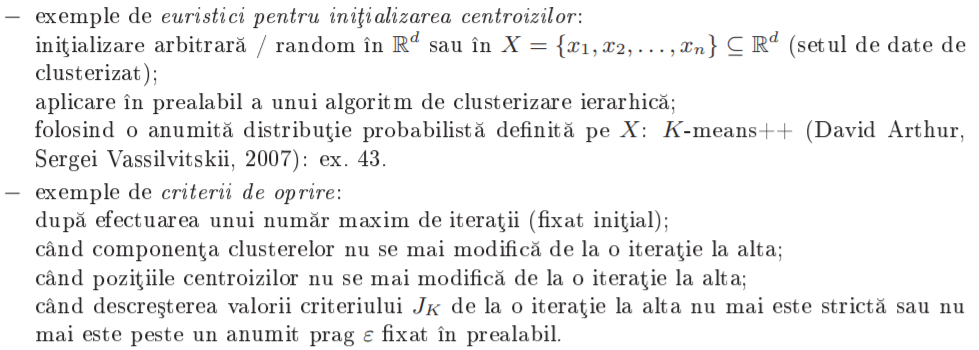
\includegraphics[width=0.8\linewidth]{screenshot001}
	\end{center}
	(preluat din \url{https://profs.info.uaic.ro/~ciortuz/ML.ex-book/book-book.8oct2019.pdf} pagina 463)
	
	Aplicare: vezi ex. 7a/pag.481 
	
	-- după cum se menționează la ex. 7a/pag.481 algoritmul poate fi aplicat în manieră \textit{\textbf{analitică}} sau \textit{\textbf{geometrică}}: vezi ex. 7a/pag.481; de fapt, atunci când aplicați k-means în manieră geometrică, la o iterație voi desenați granițele de decizie corespunzătoare algoritmului \textbf{1NN} aplicat pe centroizi: considerați fiecare centroid un punct de o anumită etichetă, iar niciun centroid nu are aceeași etichetă ca un alt centroid
	\begin{center}
		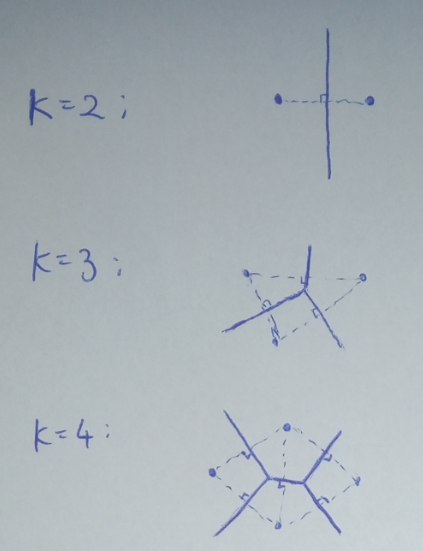
\includegraphics{screenshot002}
	\end{center}
	\newpage
	-- \textbf{granițele de separare între clustere sunt liniare}
	\begin{center}
		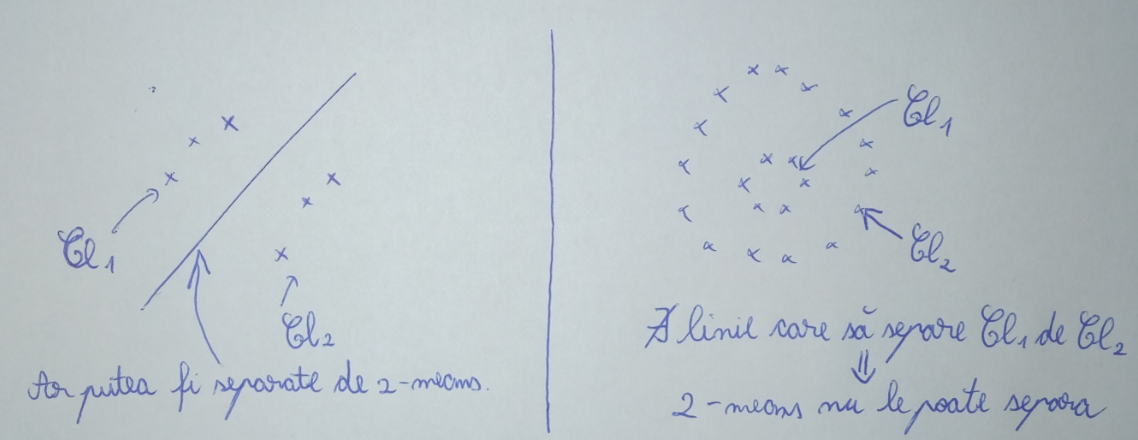
\includegraphics[width=1\linewidth]{screenshot003}
	\end{center}
	
	
	-- din cauza inițializării care poate diferi, \textbf{algoritmul nu este determinist}
	
	Două noțiuni noi:
	
	-- \textbf{k-partiție} = cele k clustere
	
	--\textbf{ k-configurație} = cei k centroizi
	
	\section{k-means - algoritm de optimizare}
	Există \textbf{două rezultate} legate de optimizare referitoare la k-means:
	\textbf{ex. 12} (este rezolvat),	\textbf{ex. 39} (este propus, dar are rezolvare în slide-uri).
	
	\subsection{Criteriul J}
	
	Pe ambele le veți aborda la curs, iar la seminar vom pune accent pe primul rezultat care spune că algoritmul k-means minimizează un \textbf{criteriu $J$ al celor mai mici pătrate}:
	\begin{align*}
	J_k(C,\mu) &= \sum_{i=1}^{n} \Vert x_i - \mu_{C(x_i)} \Vert^2
	\end{align*}
	unde $n$ reprezintă numărul de instanțe de clusterizat, $x_i$ este o instanță de clusterizat, $C$ este o împărțire a punctelor în clustere (adică o k-partiție), $\mu$ este o mulțime de \textit{reprezentanți} (vectori) pentru fiecare cluster ($\mu = (\mu_1,\dots,\mu_k)$), iar $C(x_i) \in \{1,\dots,k\}$ este clusterul la care este asignată instanța $x_i$.
	
	Altfel spus, având dat un set de date $X = (x_1,\dots,x_n)$ și un numâr natural nenul $k$, trebuie să găsim o împărțire în $k$ clustere a instanțelor și pentru fiecare cluster, un \textit{reprezentant} astfel încât criteriul $J_k(C,\mu)$ să fie minimizat. Algoritmul k-means încearcă să facă acest lucru printr-o metodă de căutare/optimizare care se numește \textbf{descreștere pe coordonate} (\textit{coordinate descent}). Astfel, k-means reușește să găsească formule de actualizare pentru $C$ și pentru $\mu$ la fiecare iterație. \textbf{Formulele pe care le găsește k-means pentru \textit{reprezentanții} $\mu$ sunt chiar formulele pentru centroizi.} Din păcate, minimul la care ajunge k-means este un \textbf{minim local}. Ex. 12/pag. 494 conține mai multe detalii legate de acest subiect.
	
	Să luăm un \textbf{exemplu de calcul pentru $J_k(C,\mu)$}. 
	
	\textbf{Exemplu}: $k = 2$, $X = (x_1,x_2,x_3)$
	
	$C_1 = \{x_1,x_2\} \Leftrightarrow$ $C(x_1) = C(x_2) = 1$, 
	
	$C_2 = \{x_3\} \Leftrightarrow C(x_3) = 2$,
	
	$\mu = (\mu_1,\mu_2)$
	
	Atunci: $J_2(C,\mu) = \Vert x_1 - \mu_1\Vert^2 + \Vert x_2 - \mu_1\Vert^2 + \Vert x_3 - \mu_2\Vert^2$ $\blacksquare$
	
	Am spus că algoritmul k-means obține un \textbf{optim local} (și nu global) pentru criteriul $J_k(C,\mu)$. Din această cauză \textbf{este bine să restartăm algoritmul cu noi valori la inițializare} și să facem acest lucru de mai multe ori; astfel, la finalul fiecărei rulări obținem câte o valoare de minim local pentru criteriul $J_k(C,\mu)$; dintre toate aceste valori putem lua valoarea minimă pentru a fi mai aproape de optimul global. Dacă, pentru un $k$ fixat, notăm cu \textbf{$J^*_k(C,\mu)$ valoarea minimă pentru $J_k(C,\mu)$ obținută după mai multe rulări}, atunci avem următoarele grafice: 
	
	\begin{center}
		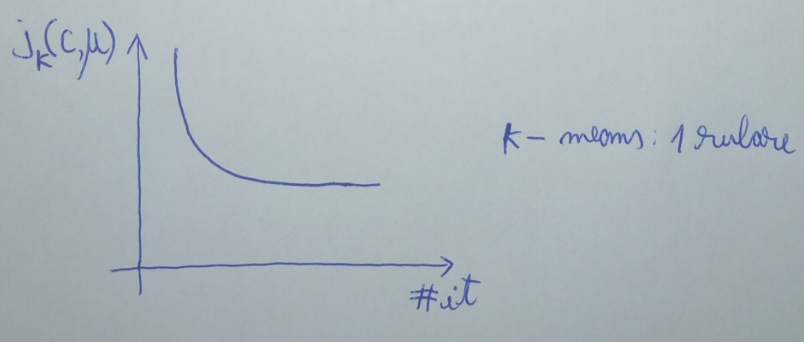
\includegraphics[width=1\linewidth]{screenshot004}
	\end{center}
	\begin{center}
		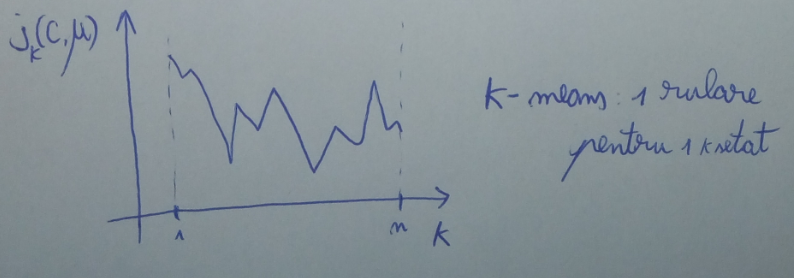
\includegraphics[width=1\linewidth]{screenshot005}
	\end{center}
	\begin{center}
		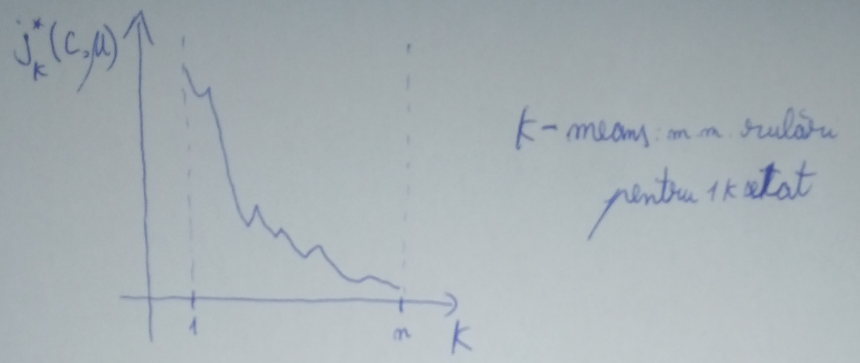
\includegraphics[width=1\linewidth]{screenshot006}
	\end{center}
	
	
	Având în vedere pașii simpli din algoritmul k-means, se mai pot defini \textbf{alte două criterii $J$}, unul care depinde doar de $\mu$ și altul care depinde doar de $C$:
	\begin{enumerate}
		\item 	$$J_k(\mu) = \sum_{i=1}^{n} \min_{j \in \{1,\dots,k\}} \Vert x_i - \mu_j \Vert^2$$
		
		\textbf{Exemplu}: $k=2$, $X=(x_1,x_2,x_3)$, $\mu = (\mu_1,\mu_2)$
		
		Atunci:
		\begin{align*}
		J_2(\mu) &= \min(\Vert x_1 - \mu_1\Vert^2,\Vert x_1 - \mu_2\Vert^2) + \\
		&+ \min(\Vert x_2 - \mu_1\Vert^2,\Vert x_2 - \mu_2\Vert^2) +\\
		&+ \min(\Vert x_3 - \mu_1\Vert^2,\Vert x_3 - \mu_2\Vert^2) \blacksquare
		\end{align*}
		
		\item 	$$J_k(C) = \sum_{i=1}^{n} \Vert x_i - \mu_j \Vert^2,$$
		unde $\mu_j = \dfrac{\sum_{x_i\in X, C(x_i) = j}x_i}{\sum_{x_i\in X, C(x_i) = j}1}$
		
		\textbf{Exemplu}: $k=2$, $X=(x_1,x_2,x_3)$, 
		
		$C_1 = \{x_1,x_2\} \Leftrightarrow$ $C(x_1) = C(x_2) = 1$, 
		
		$C_2 = \{x_3\} \Leftrightarrow C(x_3) = 2$
		
		Atunci:
		
		$\mu_1 = \dfrac{x_1 + x_2}{2}$, $\mu_2 = x_3$
		
		\begin{align*}
		J_2(C) &= \Vert x_1 - \mu_1\Vert^2 + \Vert x_2 - \mu_1\Vert^2 + \Vert x_3 - \mu_2\Vert^2 \blacksquare
		\end{align*}
	\end{enumerate}

	Observație: $J_k(C^t,\mu^{t+1}) = J_k(C^t)$, $J_k(C^t,\mu^{t}) =  J_k(\mu^{t})$, unde $C^a$ reprezintă k-partiția furnizată de k-means la iterația $a$, iar $\mu^a$ este k-configurația furnizată de k-means la iterația $a$.

	Revenind la rezultatul de la ex. 12, avem faptul că 
	
	$\underbrace{J_k(C^0,\mu^0)}_{J_k(\mu^{0})} \geq \underbrace{J_k(C^0,\mu^1)}_{J_k(C^0)} \geq \underbrace{J_k(C^1,\mu^1)}_{J_k(\mu^{1})} \geq \underbrace{J_k(C^1,\mu^2)}_{J_k(C^1)} \geq \dots$
	
	Astfel, se poate spune că algoritmul k-means nu minimiează doar $J_k(C,\mu)$, ci și $J_k(C)$, și $J_k(\mu)$. 
	
	Nu trebuie să știți toate aceste detalii, doar că în culegere când se vorbește despre criteriul $J$ se poate referi la oricare din cele trei forme de mai sus ($J_k(C,\mu), J_k(\mu), J_k(C)$). De exemplu, la ex. 13/pag. 498, este vorba despre $J_k(C)$. De ce $J_k(C)$ este interesant? Pentru că putem merge prin toate cluterizările posibile C (care sunt în număr de $k^n$, unde $k$ este numărul de clustere, iar $n$ este numărul de instanțe) și putem lua minimul. Mai mult, observăm faptul că, \textit{aproximativ}, \textbf{(mulțimea k-partițiilor lui $X$) $\subseteq$ (mulțimea (k+1)-partițiilor lui $X$)}. 
	\newpage
	De \textbf{exemplu}, dacă $X=(1,2,3)$, atunci:
	
	1-partițiile lui $X$: ($\{1,2,3\}$)
	
	2-partițiile lui $X$: 
	
	($\{\}$,$\{1,2,3\}$)
	
	($\{1\}$,$\{2,3\}$)
	
	($\{2\}$,$\{1,3\}$)
	
	($\{3\}$,$\{1,2\}$)
	
	Pentru că 1-partiția lui $X$ o putem scrie și așa: ($\{\}$,$\{1,2,3\}$), putem spune că (mulțimea 1-partițiilor lui $X$) $\subseteq$ (mulțimea 2-partițiilor lui $X$). Cu un raționament asemănător se demonstrează cazul general. $\blacksquare$
	
	Din acest motiv, dacă notăm $\underline{J}_k(C) \stackrel{\text{not.}}{=}$ \textbf{minimul global al lui} $J_k(C)$ (mergând prin toate k-partițiile posibile ale lui $X$), vom avea următorul grafic:
	\begin{center}
		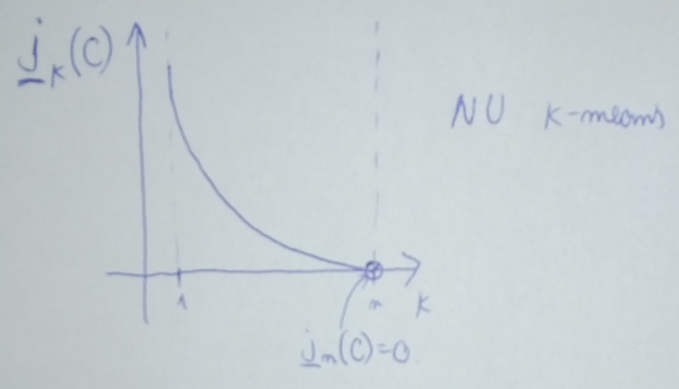
\includegraphics[width=1\linewidth]{screenshot007}
	\end{center}
	

	\subsection{k-medians}
	
	Să remarcăm faptul că în cadrul criteriului $J_k(C,\mu)$ am folosit \textbf{norma euclidiană} la pătrat. Ex. 42/pag. 546 schimbă această normă în norma cu $p=1$ și nu mai ridică la pătrat norma:
	\begin{align*}
	J_k(C,\mu)_1 &= \sum_{i=1}^{n} \Vert x_i - \mu_{C(x_i)} \Vert_1
	\end{align*}
	Astfel, având dat un set de date $X = (x_1,\dots,x_n)$ și un numâr natural nenul $k$, trebuie să găsim o împărțire în $k$ clustere a instanțelor și pentru fiecare cluster, un \textit{reprezentant} astfel încât criteriul $J_k(C,\mu)_1$ să fie minimizat. În acest caz, dacă vom deriva un algoritm în aceeași manieră în care este derivat k-means (\textit{coordinate descent}), vom da peste algoritmul k-medians. Astfel, \textbf{k-medians} reușește să găsească formule de actualizare pentru $C$ și pentru $\mu$ la fiecare iterație. \textbf{Formulele pe care le găsește k-medians pentru \textit{reprezentanții} $\mu$ nu mai sunt formulele pentru centroizi}, ci altele (pentru k-means, \textit{reprezentantul} era media unor puncte; în k-medians, \textit{reprezentantul} este mediana unor puncte). Din nou, minimul la care ajunge k-medians este un \textbf{minim local}. 

	\subsection{Ex. 39}
	
	vezi ex. 39

	\newpage
	\textbf{\large{Schemă de final}}
	\begin{enumerate}
		\item k-means - noțiuni de bază
		\item k-means - algoritm de optimizare
		\begin{enumerate}
			\item criteriul J
			\begin{enumerate}
				\item $J_k(C,\mu)$
				\item $J^*_k(C,\mu)$
				\item $J_k(\mu)$
				\item $J_k(C)$
				\item $\underline{J}_k(C)$
			\end{enumerate}
			\item k-medians
			\item ex. 39
		\end{enumerate}
	\end{enumerate}
	

	
\end{document}